\documentclass[../summary.tex]{subfiles}

\begin{document}
	
	\section{Biodiversity}
	
	\subsection{Study guide}
	
	Module 2 (Biodiversity) sketches basic insights biodiversity, different types of diversity, in an historical perspective and with options for the future. Make sure to understand:
	\begin{itemize}
		\item The different types of diversity
		\item Historical evolution of biodiversity
		\item The importance of biodiversity
		\item How can biodiversity be measured and challenges in this?
		\item The important treats for biodiversity
		\item Different options to restore biodiversity
		\item Being able to interpret data with regard to biodiversity
	\end{itemize} 
	
	Don’t learn the specific examples by heart, do not learn specific vocabulary by heart (such as Cambrian or Cretaceous).
	\\
	
	\subsection{Types of diversity}
	The variability among living organisms from all sources, including, inter alia, terrestrial, marine and other aquatic ecosystems and the ecological complexes of which they are parts. This includes the diversity within species, between species and of ecosystems
	
	The first type of biodiversity is genetic diversity or diversity between species. It is the amount of naturally occurring genetic variation among individuals of the same species. 
	\\
	Another type of diversity is species diversity. This type is often defined as the number of species at a certain location. Figure \ref{fig:diversity_species} gives an indication of this diversity.
	\begin{figure}[htbp]
		\centering
		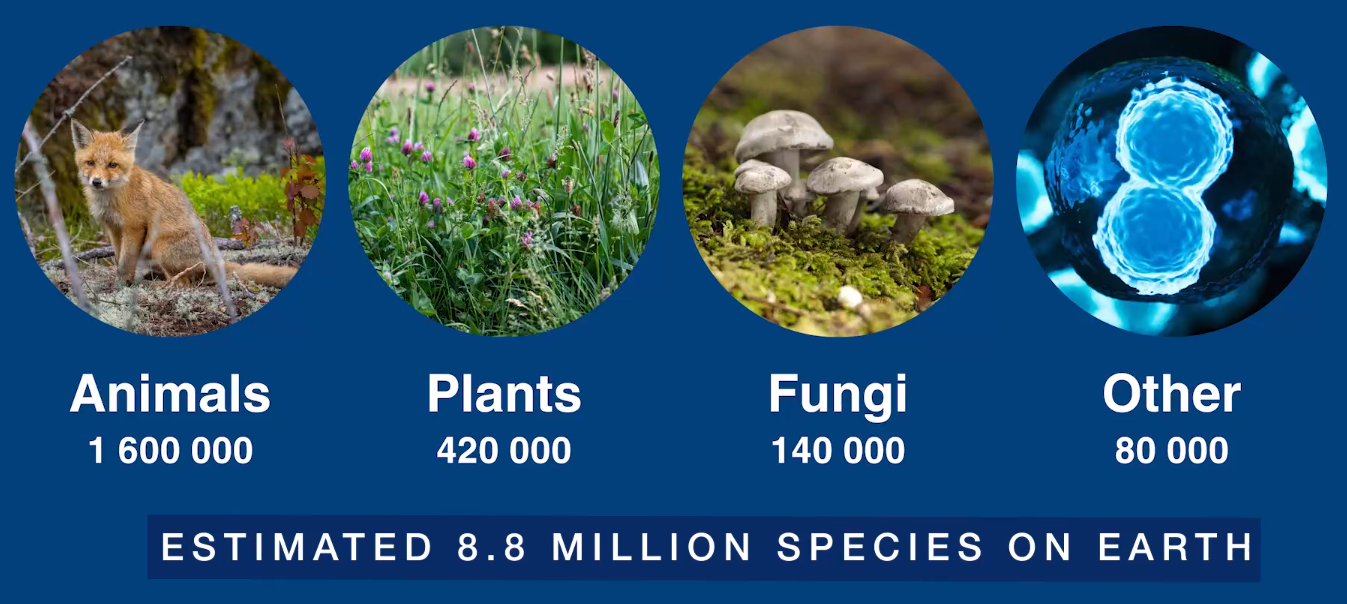
\includegraphics[width=1\linewidth]{images/2-diversity_species.png}
		\caption{Diversity in species}
		\label{fig:diversity_species}
	\end{figure}
	\\
	Thirdly, there also is diversity in ecosystems. There are a lot of different ecosystems around the globe: from the boreal forest at high latitudes to tropical forests around the equator, but also aquatic ecosystems like lake systems, coral reefs and mangroves count towards ecosystem diversity.
	
	\subsection{Historical evolution of biodiversity}
	
	\subsection{The importance of biodiversity}
	In the Ecosystem Services cascade of figure \ref{fig:ecosystems_services_cascade}, we see the integrated social-ecological system with to the left the ecosystem and to the right the human society. The ecosystem has its composition, structure and function, which all are determined by its biodiversity. The human society receives a flow of ecosystem services from the ecosystem, which contribute to the prosperity and well-being of its members. Ecosystem Services are the goods and services humans get from ecosystems and can be divided in three main categories: provisioning, regulating and cultural services. The provisioning services consist of the material flows, like agricultural crops for food, wood for construction, biomass for energy or drinking water. Regulating services are those that provide environmental protection like erosion control, air cooling and filtering by vegetation or climate mitigation through carbon uptake and storage in forests, peatlands and soils. Cultural services include the diverse spiritual, recreational and scientific experiences ecosystems provide to humans. All these services directly depend on biodiversity.
	\begin{figure}[htbp]
		\centering
		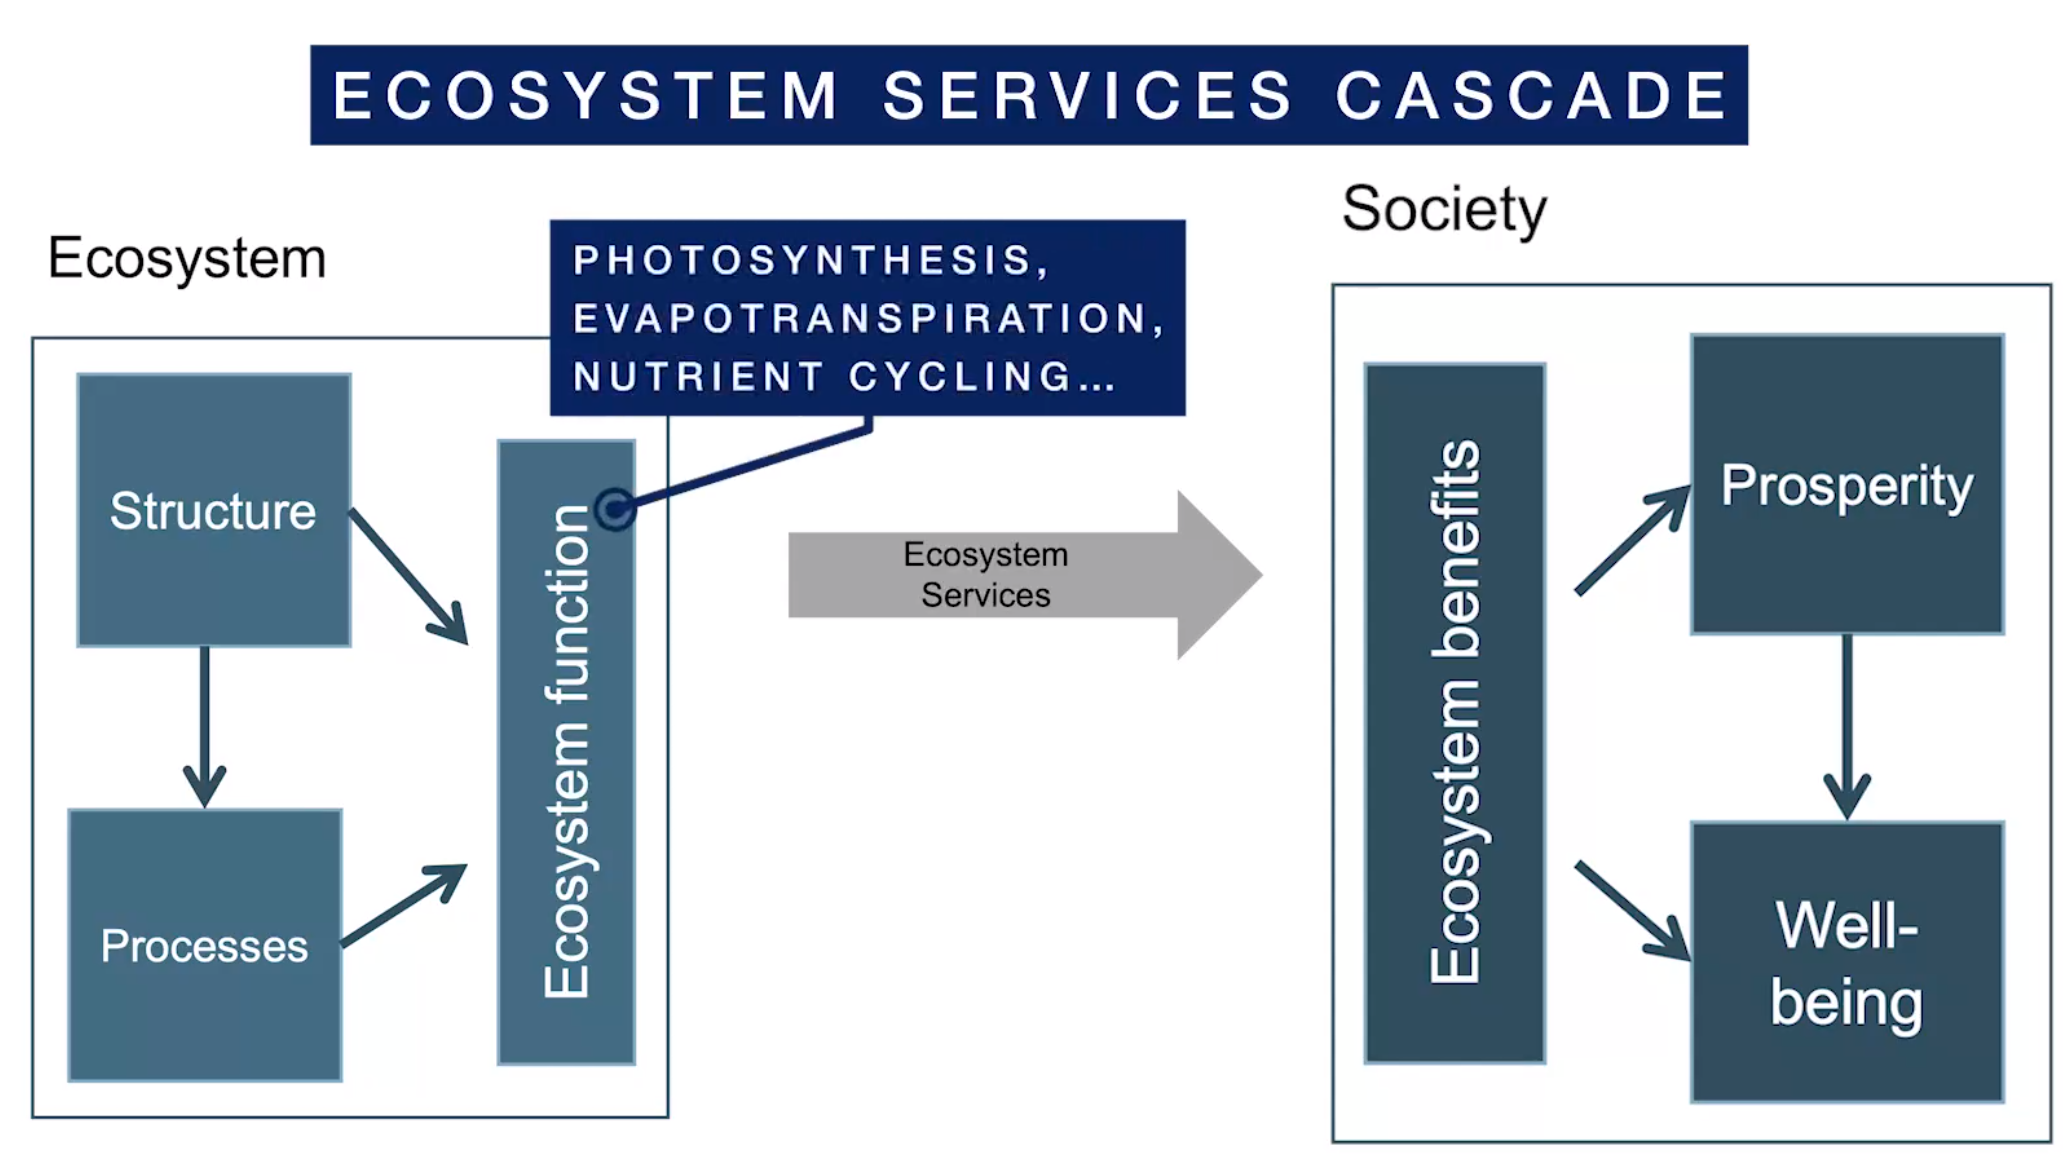
\includegraphics[width=1\linewidth]{images/2-ecosystem-services-cascade.png}
		\caption{Ecosystem Services cascade}
		\label{fig:ecosystems_services_cascade}
	\end{figure}
	\\
	There is a positive but asymptotic biodiversity – ecosystem service relationship. This relationship is visualised in figure \ref{fig:relationship_biodiversity_ecosystems_services}. This means that increasing biodiversity leads to an increase in ecosystem service performance up to a certain extent, after which adding more biodiversity does not much further increase the service provision. It also means that losing some biodiversity as a consequence of human ecosystem degradation may not directly lead to large losses in ecosystem services, but that a further degradation over a critical threshold of species loss will lead to strong reductions in ecosystem services.
	\begin{figure}[htbp]
		\centering
		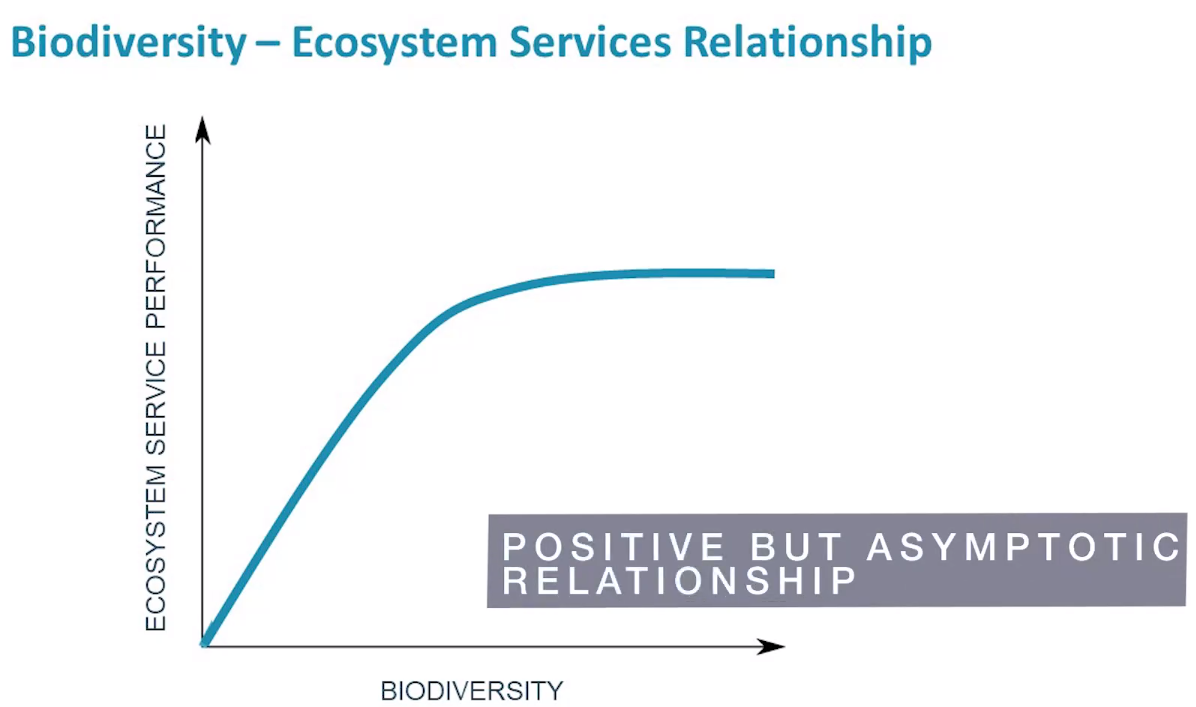
\includegraphics[width=1\linewidth]{images/2-biodiversity-ecosystem-services-relationship.png}
		\caption{Relationship between biodiversity and ecosystems services}
		\label{fig:relationship_biodiversity_ecosystems_services}
	\end{figure} 
	\\
	
	
	\subsection{Measuring of biodiversity}
	
	\subsection{Treats for biodiversity} 

	\subsection{Restoring biodiversity}

	
	
	
	
\end{document}